\documentclass[12pt]{article}
\usepackage{setspace, graphicx, fullpage, amssymb, amsmath, epsfig, natbib, array, multirow, hyperref}
\usepackage{amsfonts, bm} 
\usepackage{dcolumn}
\usepackage{subfigure, float} 
\usepackage[margin=1in]{geometry} 
\usepackage{verbatim}
\usepackage{url}
\usepackage{enumerate}
\usepackage{morefloats}
\newcolumntype{d}[1]{D{.}{.}{#1}} 



\begin{document}
	
\begin{center}
	\Large 22 March 2017
\end{center}

\section{Overview}

At our previous meeting we decided to do the following:
\begin{itemize}
	\item Rewrite sections of the first draft in order to better describe what the contribution of Minozzi \& Volden (2013) was in order to frame our replication, enter more fully into the conversation on elections and induced preferences, and discuss the fact that on non-party calls extremists walk away from the party just like moderates.
	
	\item Develop coefficient plots to replace the tables for the diff-in-diff/coherence design
	
	\item Write appendices which cover differences from the House sorting model and the reelection matching
	
	\item Write a single R script which creates all the tables and figures we are considering using in this paper
	
	\item Create a separate \LaTeX document which contains tables and figures we would want to include in a second paper focused on increases in party calls over Congresses 93-112
\end{itemize}

\section{Paper, Draft 2}

\subsection{Introduction}

Minozzi \& Volden (2013) showed that the typical view of Congressional parties offering personal benefits to moderates in order to achieve unity on key bills was not capturing most of what happens in order to meet the party's needs. Instead, much of what happens in order to achieve partisan goals entails appeals to benefit the brand name of the party. While an improved party brand improves the fortunes of all members, members must gain differentially from the party itself and their perceived relationship to it. More extreme members in the party were hypothesized and shown to be the most responsive to a party call because they gain the most both from the status of the party and their status as a partisan in most cases. Extreme members who already have strong preferences on an issue would be unlikely to see this preference change, but those whose preferences are weaker will see the call as a clear reason to align for the good of the party.

This paper works to replicate these findings and extend them into more recent Congresses (110-112) in the House as well as into the Senate for these Congresses. This allows us to test the responsive extremists hypothesis in times that the party is thought to be getting more extreme in the House. We can also test if it holds when applied to the Senate in order to see if it is a quirk of the House or a trait of Congressional behavior generally. We hypothesize that these relationships will be largely the same. Further, the inclusion of the Senate allows us to consider the influence of proximity to reelection in choosing whether to heed the call of the party.

Mayhew (1974) shows that reelection is chief among the desires of members of Congress. Canes-Wrone, Brady \& Cogan (2002) shows that members who stray to far from the preferences of their district are less likely to be reelected. While this would initially seem to imply that members would act according to the preferences of their district above those of their party, we know from Lee (2009) that the name brands of parties confer advantages on members and that members are thus willing to take actions and positions that are either beneficial to their own party relative to the opposition. and Carson, Koger, Lebo \& Young (2010) that following the party line too closely can in itself be electorally costly to an individual member. Levitt (1996) finds that proximity to reelection induces Senators to more strongly take their constituents' preferences into account.

In particular, Levitt has the most implications for the responsive extremists hypothesis. If members only respond to party calls when they do not have strong preferences against the party and proximity to reelection increases the attention they pay to their constituents' preferences, we should expect that members will be less responsive to party calls in Congresses which they are up for reelection.

\subsection{Replication with Extension}

In this section we show that the results from Minozzi \& Volden (2013) hold when analysis is extended into later Congresses and the Senate. We draw on Congressional roll call data for Congresses 93-112 for both chambers in order to view the behavior of members. As in Minozzi \& Volden (2013), we iteratively sort votes based on the the predictive power of party in vote decision taken alongside party free ideology. We dub those votes which are significantly predicted by party as party calls and those which are not as noncalls. The set of noncalls from one iteration is used as the votes for calculating party free ideology in the next. A more thorough overview of the original algorithm and the changes we've made to it are detailed in an appendix.

We make a number of important findings. First, the relationship between extremism and vote choice is not random with both extremists and moderates of each party likely to vote against the party on non party call votes, but on party call votes the extremists snap intoline with the party. The relationship we find between ideological extremism and party call responsiveness, shown in figures 1 and 2 demonstrates this as a percent. The nonlinearity between party call response rate and ideological extremism appears to arise from the fact that there is a maximum rate of 100\%.

\begin{figure}[H]
	\centering
	\caption{House Rate of Voting With Party by Vote Type}
	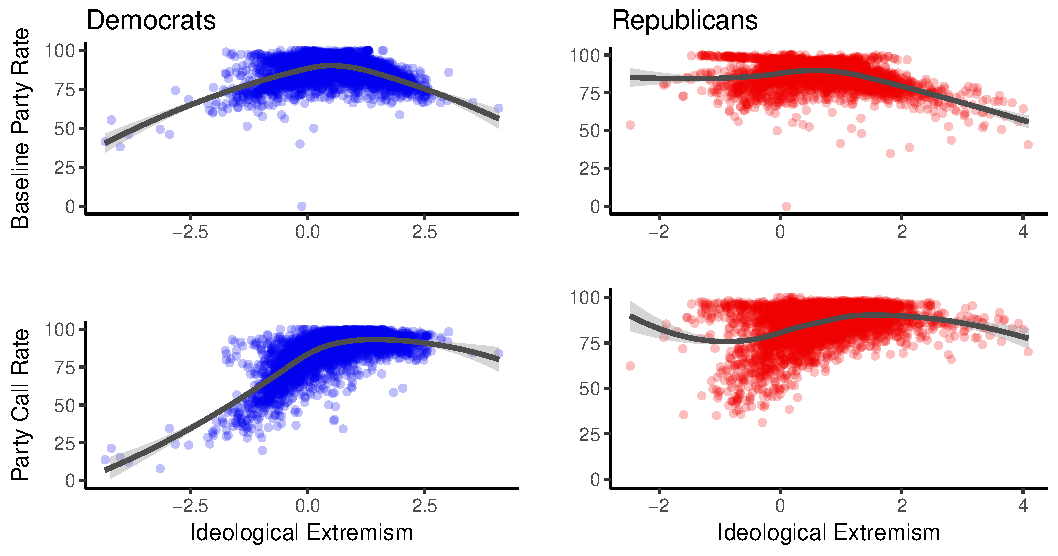
\includegraphics[width = 10cm]{C:/Users/Ethan/Documents/GitHub/partycalls/plots/house_responsiveness_plot.pdf}
\end{figure}

\begin{figure}[H]
	\centering
	\caption{Senate Rate of Voting With Party by Vote Type}
	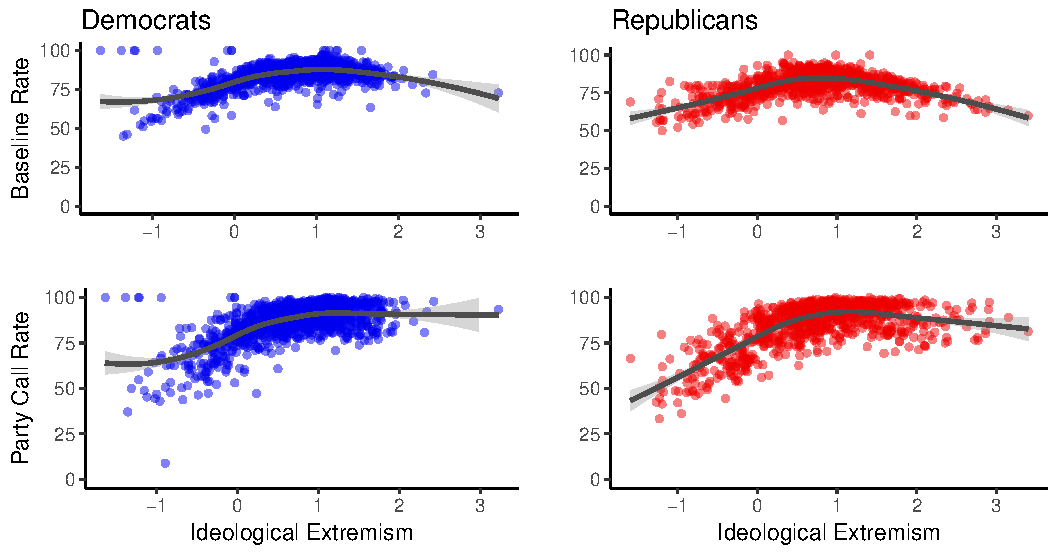
\includegraphics[width = 10cm]{C:/Users/Ethan/Documents/GitHub/partycalls/plots/senate_responsiveness_plot.pdf}
\end{figure}

Further, pooled regressions with members divided by party and majority status broadly show similar relationships both between chambers in the current analysis as well as with those presented in Minozzi \& Volden (2013). Though they differ in strength between parties, ideological extremism and rate of voting with majority of non party call votes both carry substantive predictive power in determining responsiveness by to party calls. 

Unsurprisingly, in both chambers we also find that southern Democrats are less responsive to the party than are other Democrats. We also note that the power committee variable we constructed for the Senate (based on membership in a top 4 committee) carries little predictive power, either in terms of substantive power or statistical significance. This is unsurprising since this is a variable we included less because we believed it had meaning to Senators and more for model comparability. We also note that in both chambers increased same party presidential vote share within one's constituency makes Democrats more likely to respond to a party call but reduces the chances of a Republican doing so.

\begin{table}
	\begin{center}
		\caption{House Responsiveness to Party Calls, Pooled Regressions}
		\begin{tabular}{l c c c c }
			\hline
			& Democrats & Republicans & Majority & Minority \\
			\hline
			Ideological Extremism & $8.338^{***}$  & $5.845^{***}$  & $6.650^{***}$  & $8.730^{***}$  \\
			& $(0.168)$      & $(0.207)$      & $(0.157)$      & $(0.200)$      \\
			Baseline Rate of Voting with Party              & $0.637^{***}$  & $0.414^{***}$  & $0.520^{***}$  & $0.635^{***}$  \\
			& $(0.015)$      & $(0.020)$      & $(0.015)$      & $(0.020)$      \\
			Vote Percent                & $-0.036^{***}$ & $-0.005$       & $-0.087^{***}$ & $-0.066^{***}$ \\
			& $(0.009)$      & $(0.013)$      & $(0.009)$      & $(0.012)$      \\
			Pres. Vote Share          & $0.092^{***}$  & $-0.087^{***}$ & $0.196^{***}$  & $0.165^{***}$  \\
			& $(0.011)$      & $(0.019)$      & $(0.011)$      & $(0.017)$      \\
			South                  & $-2.431^{***}$ & $3.628^{***}$  & $-1.638^{***}$ & $-0.376$       \\
			& $(0.280)$      & $(0.336)$      & $(0.250)$      & $(0.315)$      \\
			Female                 & $0.529$        & $-0.081$       & $-0.142$       & $2.122^{***}$  \\
			& $(0.354)$      & $(0.575)$      & $(0.403)$      & $(0.442)$      \\
			African American                   & $-0.522$       & $5.014$        & $-3.039^{***}$ & $3.252^{***}$  \\
			& $(0.440)$      & $(2.974)$      & $(0.534)$      & $(0.607)$      \\
			Latino                 & $1.732^{***}$  & $2.415^{*}$    & $2.824^{***}$  & $3.022^{***}$  \\
			& $(0.514)$      & $(1.154)$      & $(0.626)$      & $(0.704)$      \\
			Seniority              & $0.048$        & $-0.329^{***}$ & $0.013$        & $0.007$        \\
			& $(0.031)$      & $(0.050)$      & $(0.034)$      & $(0.041)$      \\
			Freshman               & $-0.071$       & $1.001^{*}$    & $0.235$        & $-0.410$       \\
			& $(0.357)$      & $(0.462)$      & $(0.347)$      & $(0.446)$      \\
			Best Committee          & $-0.039^{*}$   & $-0.237^{***}$ & $-0.175^{***}$ & $-0.162^{***}$ \\
			& $(0.019)$      & $(0.025)$      & $(0.019)$      & $(0.023)$      \\
			Party Leader                 & $1.957^{**}$   & $2.795^{***}$  & $2.615^{***}$  & $1.783^{**}$   \\
			& $(0.599)$      & $(0.761)$      & $(0.646)$      & $(0.653)$      \\
			Power Committee                  & $1.816^{***}$  & $2.951^{***}$  & $3.017^{***}$  & $1.058^{**}$   \\
			& $(0.275)$      & $(0.374)$      & $(0.268)$      & $(0.361)$      \\
			Committee Chair                  & $2.491^{***}$  & $9.848^{***}$  & $1.864^{***}$  &                \\
			& $(0.498)$      & $(0.803)$      & $(0.443)$      &                \\
			(Intercept)            & $23.996^{***}$ & $53.041^{***}$ & $36.446^{***}$ & $17.692^{***}$ \\
			& $(1.576)$      & $(2.206)$      & $(1.489)$      & $(2.050)$      \\
			\hline
			R$^2$                  & 0.631          & 0.303          & 0.566          & 0.478          \\
			Adj. R$^2$             & 0.630          & 0.300          & 0.565          & 0.476          \\
			Num. obs.              & 4746           & 3798           & 4898           & 3646           \\
			RMSE                   & 7.365          & 8.870          & 7.543          & 8.022          \\
			\hline
			\multicolumn{5}{l}{\scriptsize{$^{***}p<0.001$, $^{**}p<0.01$, $^*p<0.05$}}
		\end{tabular}
	\end{center}
\end{table}

\begin{table}[H]
	\begin{center}
		\caption{Senate Responsiveness to Party Calls, Pooled Regressions}
		\begin{tabular}{l c c c c }
			\hline
			& Democrats & Republicans & Majority & Minority \\
			\hline
			Ideological Extremism & $3.136^{***}$  & $7.792^{***}$   & $4.708^{***}$  & $7.949^{***}$ \\
			& $(0.409)$      & $(0.357)$       & $(0.315)$      & $(0.400)$     \\
			Baseline Rate of Voting with Party              & $0.759^{***}$  & $0.742^{***}$   & $0.702^{***}$  & $0.702^{***}$ \\
			& $(0.030)$      & $(0.031)$       & $(0.025)$      & $(0.035)$     \\
			Up For Reelection    & $-0.630$       & $-1.436^{**}$   & $-0.951^{*}$   & $-1.204^{*}$  \\
			& $(0.426)$      & $(0.538)$       & $(0.411)$      & $(0.603)$     \\
			Vote Share            & $-0.053^{*}$  & $0.149^{***}$  & $-0.012$       & $0.076^{*}$   \\
			& $(0.022)$     & $(0.028)$      & $(0.021)$      & $(0.030)$     \\
			Presidential Vote Share       & $0.234^{***}$ & $-0.134^{***}$ & $0.182^{***}$  & $0.006$       \\
			& $(0.024)$     & $(0.031)$      & $(0.020)$      & $(0.032)$     \\
			South                  & $-1.690^{**}$  & $0.872$         & $0.054$        & $1.085$       \\
			& $(0.557)$      & $(0.578)$       & $(0.427)$      & $(0.622)$     \\
			Female                 & $1.690^{*}$    & $0.451$         & $0.532$        & $4.256^{***}$ \\
			& $(0.730)$      & $(1.132)$       & $(0.758)$      & $(1.113)$     \\
			African American                   & $-1.164$       & $-10.789^{*}$   & $1.531$        & $-5.519$      \\
			& $(2.789)$      & $(4.278)$       & $(4.184)$      & $(3.219)$     \\
			Latino                 & $1.814$        & $7.264^{**}$    & $4.781^{*}$    & $6.253$       \\
			& $(2.198)$      & $(2.779)$       & $(1.878)$      & $(3.506)$     \\
			Seniority              & $0.041$        & $-0.024$        & $0.077$        & $0.118$       \\
			& $(0.052)$      & $(0.072)$       & $(0.060)$      & $(0.070)$     \\
			Freshman               & $0.769$        & $0.358$         & $0.600$        & $0.996$       \\
			& $(0.708)$      & $(0.842)$       & $(0.631)$      & $(1.032)$     \\
			Retiree                & $1.599$        & $2.290^{*}$     & $1.816^{*}$    & $2.575^{*}$   \\
			& $(0.897)$      & $(0.997)$       & $(0.850)$      & $(1.110)$     \\
			Best Committee        & $0.237$        & $0.008$         & $0.027$        & $0.373^{*}$   \\
			& $(0.124)$      & $(0.154)$       & $(0.118)$      & $(0.174)$     \\
			Party Leader                 & $2.218^{**}$   & $0.910$         & $1.441^{*}$    & $1.940^{*}$   \\
			& $(0.712)$      & $(0.776)$       & $(0.661)$      & $(0.899)$     \\
			Power Committee       & $-0.855$       & $-0.325$        & $-0.052$       & $-1.468$      \\
			& $(0.772)$      & $(0.924)$       & $(0.719)$      & $(1.064)$     \\
			Chair                  & $0.852$        & $3.626^{***}$   & $-0.017$       &               \\
			& $(0.543)$      & $(0.700)$       & $(0.517)$      &               \\
			(Intercept)            & $9.447^{**}$   & $18.182^{***}$  & $16.365^{***}$ & $10.799^{**}$ \\
			& $(2.906)$      & $(3.489)$       & $(2.644)$      & $(4.009)$     \\
			\hline
			R$^2$                  & 0.689          & 0.641           & 0.684          & 0.615         \\
			Adj. R$^2$             & 0.684          & 0.635           & 0.679          & 0.608         \\
			Num. obs.              & 1042           & 951             & 1052           & 843           \\
			RMSE                   & 6.118          & 7.255           & 5.865          & 7.749         \\
			\hline
			\multicolumn{5}{l}{\scriptsize{$^{***}p<0.001$, $^{**}p<0.01$, $^*p<0.05$}}
		\end{tabular}
	\end{center}
\end{table}

In Table 2, we see some evidence of differences between members up for reelection and others. Though it fails to meet traditional significance threshold for Democrats, across all subgroups this coefficient is negative. 

\subsection{Reelection in the Senate}

In this section we estimate models which account for variation within members. The first tests compare the effects of being up for reelection on responsiveness to party calls and baseline rate of voting with the party through a non-parametric test. This test approximates a difference in differences test, relying on same-state Senator pairs with one member of the pair up for reelection and one not. We report these in separate tables which contain an estimated effect as well as the upper and lower bounds of 95\% bootstrapped confidence intervals for the reelection treatment and a randomly assigned ``placebo'' treatment. No controls are included in these models beyond comparison of same-state Senators. 

We use these tests to show that member behavior differs meaningfully in regard to party call votes and not noncall votes when they are up for reelection. The strength of this relationship is consistent with that found among groups (other than Democrats) in the pooled regressions found in the previous section.


\subsection{Conclusion}

\section{Appendices}

\subsection{Appendix A: Detailing the New Sorting Algorithm}

We have made some changes to the sorting algorithm used to sort votes. One of the key changes was the use of the \verb|emIRT()| R function as described in Imai, Lo \& Olmsted (2016) in order to obtain members' party free ideology. This function was developed by those authors in order to produce estimates analagous to those of the \verb|ideal()| function developed by Clinton, Jackman \& Rivers (2004) and used in the prior party call sorting algorithm. A key advantage of this new function for estimation of member ideology is that it produces results with greatly reduced computation. These and other changes, as detailed in an appendix, produce highly similar results to those found in Minozzi \& Volden (2013) when applied to both chambers. We find for each chamber that party call votes are more often close votes and the opposite holds for noncalls. Votes are considered lopsided when at least 65\% of members vote the same way on it and close otherwise.

\subsection{}

% latex table generated in R 3.3.2 by xtable 1.8-2 package
% Sun Mar 26 19:10:24 2017
\begin{table}[H]
	\centering
	\caption{Reelection and Response to Party Calls, Difference in Differences} 
	\begin{tabular}{llrrr}
		\hline
		test & DV & Estimate & Lower\_Bound & Upper\_Bound \\ 
		\hline
		Effect & pirate100 - pfrate100 & -1.272 & -1.775 & -0.794 \\ 
		Placebo & pirate100 - pfrate100 & -0.292 & -0.904 & 0.935 \\ 
		\hline
	\end{tabular}
\end{table}

% latex table generated in R 3.3.2 by xtable 1.8-2 package
% Sun Mar 26 19:10:27 2017
\begin{table}[H]
	\centering
	\caption{Diff in Diff, Subgroup Condition, Party Influenced Rate} 
	\begin{tabular}{llr}
		\hline
		Test & DV & Estimate \\ 
		\hline
		2 Maj Dems Effect & pirate100 - pfrate100 & -0.1191943 \\ 
		2 Maj Dems Placebo & pirate100 - pfrate100 & 0.5657017 \\ 
		2 Min Dems Effect & pirate100 - pfrate100 & -1.8253378 \\ 
		2 Min Dems Placebo & pirate100 - pfrate100 & -0.4463733 \\ 
		2 Maj Reps Effect & pirate100 - pfrate100 & -2.2112471 \\ 
		2 Maj Reps Placebo & pirate100 - pfrate100 & -0.1749949 \\ 
		2 Min Reps Effect & pirate100 - pfrate100 & 0.7774782 \\ 
		2 Min Reps Placebo & pirate100 - pfrate100 & -0.4516436 \\ 
		Split, Maj Dem, Dem Effect & pirate100 - pfrate100 & -0.8756821 \\ 
		Split, Maj Dem, Dem Placebo & pirate100 - pfrate100 & -1.8454871 \\ 
		Split, Maj Dem, Rep Effect & pirate100 - pfrate100 & -1.4582552 \\ 
		Split, Maj Dem, Rep Placebo & pirate100 - pfrate100 & 0.0117995 \\ 
		Split, Maj Rep, Dem Effect & pirate100 - pfrate100 & -7.1166813 \\ 
		Split, Maj Rep, Dem Placebo & pirate100 - pfrate100 & -3.4630959 \\ 
		Split, Maj Rep, Rep Effect & pirate100 - pfrate100 & 0.3772151 \\ 
		Split, Maj Rep, Rep Placebo & pirate100 - pfrate100 & 0.2964502 \\ 
		\hline
	\end{tabular}
\end{table}




























































\end{document}